%!TEX root = ../report.tex
%%%%%%%%%%%%%%%%%%%%%%%%%%%%%%%%%%%%%%%%%%%%%%%%%%%%%%%%%%%%%%%%%%%%%%%
%%%%%%%%%%%%%%%%%%%%%%%%%%%%%%%%%%%%%%%%%%%%%%%%%%%%%%%%%%%%%%%%%%%%%%%
%%%%%                                                                 %
%%%%%     06_implementation.tex                                       %
%%%%%                                                                 %
%%%%% Author:      Florian Zaruba                                     %
%%%%% Created:     13.12.2015                                         %
%%%%% Description: <description>                                      %
%%%%%                                                                 %
%%%%%%%%%%%%%%%%%%%%%%%%%%%%%%%%%%%%%%%%%%%%%%%%%%%%%%%%%%%%%%%%%%%%%%%
%%%%%%%%%%%%%%%%%%%%%%%%%%%%%%%%%%%%%%%%%%%%%%%%%%%%%%%%%%%%%%%%%%%%%%%


\chapter{Design Implementation and Results}

This chapter is about the implemented functionality and ASIC key design data (timing, area and power) and implementation decisions made.

\section{Implementation}

\subsection{Multiplexed Pads}

Since pads are often a quite limiting factor in the overall design it can be particularly useful to reuse them depending on the functionality required at a certain point in time.

The pads should remain highly configurable. Therefore it was necessary to multiplex all inputs and outputs of every pad instance that should perform a secondary function (for example function as an UART or GPIO). Depending on a configuration register in the APB \pulpino Peripheral (\ref{subsec:pulpino_peripheral}) the pad should switch functionality. In addition all pads need to be in a fixed configuration when the chip is on the tester (testmode is enabled).

The block diagram of the pad multiplexers is depicted in figure~\ref{fig:pad_muxes}. In order to not clutter the circuit diagram too much output enable, input, output and configuration multiplexers are drawn for different functionality of the circuit. In fact all pins that share functionality feature all multiplexers depicted.
\begin{itemize}
    \item \textbf{Output Enable (OE)}: For the pads primary function output is either tied to low or high depending on the main functionality. If the pad is configured as general purpose I/O it is connected to the configuration register of the APB GPIO module (see~\ref{subsec:gpio_peripheral}).
    \item \textbf{Input}: If the pad serves double functionality, in terms of that its primary function serves as input, its input pin is multiplexed to the main entity. Depending on how the pad is currently configured the the non-active input is silenced.
    \item \textbf{Output}: If the pad serves as an output in its primary function the output to the pad is selected in terms of its current configuration.
    \item \textbf{Pad Config}: Pad configuration is a 6 bit wide bus that sets the pads configuration, depending on its current functionality, accordingly (like Schmitt Trigger, Drive Strength, etc.).
\end{itemize}
An exhaustive pad list along with reset configuration values is depicted in the chip's data-sheet (\ref{tab:pads})).


\begin{figure}[tbh]
  \centering
  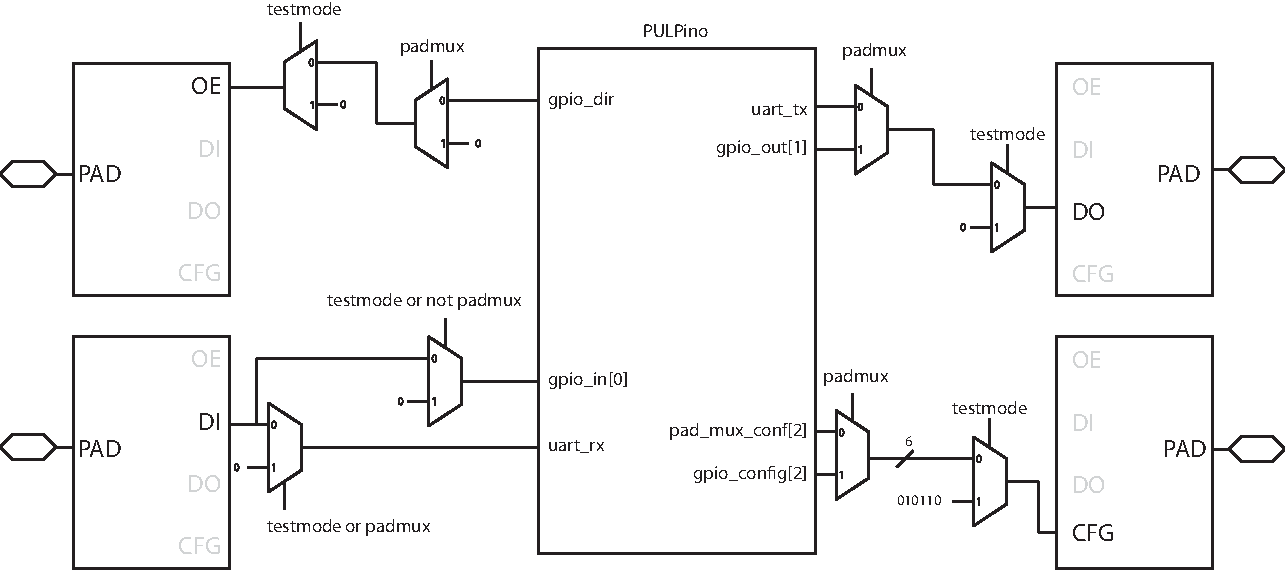
\includegraphics[width=\linewidth]{./figures/pad_muxes}
  \caption{Multiplexed Pads}
  \label{fig:pad_muxes}
\end{figure}

\subsection{Register file}
% Latch based vs. register based register file
\pulpino provides to different implementation for its register file. One is standard array of flip-flops while the other makes use of clock gated latches. The first one has the advantage of being a very simple design choice that performs well in classical verification methods like Scan-Chain insertion but has the disadvantage of having an area overhead compared to the latch based register file.

As mentioned above the latch base register file is smaller and dissipates less power than the flip-flop based approach but isn't as, at least with classic full scan insertion, well testable as the flip-flop version. 

To have a comparison of the two approaches I synthesized both versions and did automatic test pattern generation (ATPG) with TetraMax.

\begin{figure}[ht!]
\centering
\begin{tabularx}{\textwidth}{Xrr}
  \textbf{Type} & \textbf{Area} (\textmu$m^2$) & \textbf{Test} \textbf{Coverage} (\%) \\  \hline
  latch based register file & $8541$ & $86.2$  \\
  flip-flop based register file & $12278$ & $97.2$\\
\end{tabularx}
\caption{Comparison of latch based and flip-flop based register file (test coverage vs. area)}
\label{tab:reg_file}
\end{figure}

As you can see in table~\ref{tab:reg_file} swapping the latch based register file for a flip-flop version results in an area overhead of about 1.44 opposed to the latch based version, but results in a significant better test coverage.

\subsection{RAM banks}
%relate to timing

\section{Booting}
\label{sec:booting}

Booting is an essential part of the ASIC implementation. Unless you are really accounting for loading program data into the microcontroller you are left with a worthless piece of silicon. 

\subsection{Booting from ROM}
The boot process on Imperio is achieved by a 2 kByte of boot ROM that has instructions that read a SPI Flash and load the program's instructions and data into memories.

The compiled program is stored in the SPI Flash. It starts at address zero with 32 bytes of meta data that tell the bootcode where the instruction section begins, how many bytes are used to encode each instruction, where it should start fetching and how may blocks of fixed length it has to expect. The same is done for the data.

A special script takes care of preparing the flash content. This means calculating the headers and formatting the instructions.

The core starts executing boot code unless otherwise explicitly told so by writing the start address registers in the \pulpino APB peripheral (see~\ref{subsec:pulpino_peripheral})). 

The boot sequence starts by reading the vendor ID of the connected SPI Flash (we are only supporting a certain type of SPI Flash, where we definitely know all timing parameters). Next the SPI Master switches the communication to Quad SPI which is an extension to standard SPI but with 4 bidirectional data lanes. This has the advantage of providing a speedup of four times.

Next, the processor reads the 32 byte of header information and starts by loading instruction data into its instruction RAM. Afterwards the same is done for the data section of the program. Finally it jumps to the base of the instruction RAM and starts executing the main program.

During the boot process interrupts are disabled and all peripherals except the SPI Master are in reset configuration. For the full boot code refer to~\ref{sec:boot_code}.

\subsection{Booting over SPI or JTAG}

Since the SPI Slave and the JTAG port of the ADU have access to the bus it is possible to store external data into the RAMs. This in fact can be used and is actually intended to give a way of loading an entrire program into Imperio's RAMs.


\section{Verification}

This section deals with functional and circuit level verification. In the functional section I will give detailed explanation on how \pulpino and Imperio are tested.

\subsection{Functional}

For functional verification we mainly distinguish two test settings: \pulpino related functional verification and imperio related verification. One can see Imperio's test setting as superset of \pulpino's e.g. every test that can be run on \pulpino can also be conducted on Imperio but not vice-verse.

\subsubsection{\pulpino testbench}

\pulpino tests are performed in a platform setting. This means that the core gets instantiated in the target platform setting and is then tested exclusively in this environment. This provides the advantage of having a very generic test framework which allows us to test (high level) assembly and C code. We have a specialized test library in place that performs checks for errors and generates reports that are output over UART. Currently we are supporting two different kind of tests:
\begin{enumerate}
    \item \textbf{Sequential Tests:} Pure C code tests that perform common micro-benchmarks like sorting, matrix multiplication.
    \item \textbf{RISC-V Tests:} Test that are exercising certain features of the core. This group also contains Berkely's official RISC-V tests that have been ported in the course of RI5CY's development. Additionally we are testing load/stores, control flow instructions and our instruction set extensions amongst others.
\end{enumerate}

The testbench is highly configurable through parameters that are set when the corresponding testbench script is invoked (see the \verb+vsim/scripts+ folder for a list of available configurations see~\ref{subsec:directory_structure}). I want to emphasize two particular configuration parameters namely clock select and memload. 

The first one selects whether the core should be clocked by an external reference clock or by its internal FLL. In terms of RTL simulation this does not matter too much since we do not have any timing parameters that may prevent us to use higher clock speeds through the external clock generation. But it allows for functional verifying the FLL.

The memload parameters specifies how the memories of the DUT should be filled with instructions and data. For \pulpino we support:
\begin{itemize}
    \item \textbf{Memory pre-loading}: In this setting we make use of the fact that we can directly pre-load the memories' functional model. Prior to starting the core all memories are filled with the content of \verb+.slm+ files that have been created of the corresponding object file with special conversion scripts (located in \verb+sw/utis/+).
    \item \textbf{SPI Slave}: As discussed in the SPI Slave Section (\ref{subsec:spi_slave}) \pulpino's entire memory region can be written from outside via SPI. This makes it possible to load instructions and data through SPI.
    \item \textbf{JTAG}: Since the whole memory region is mapped to a common address space it is possible to write the RAMs through JTAG as well. Therefore it is possible to load a program via JTAG.
\end{itemize}

After the program has been loaded by either of the three possibilties specified above the fetch enable signal gets asserted and the core start computation. Depending on the test currently running the results are checked against a different golden model. This can either be some constants that where computed prior to compilation or other entities that get checked, for example a certain register's content. 

Once the test passes this check, the result is reported back to the test bench library that outputs a predefined string over UART and signals the end of computation (EOC) event by pulling GPIO 8 high. Depending on the environment the test is running this string either gets checked manually or automatically by the \verb+run_and_check.py+ python script.

One particular point I'd like to stress is that it is necessary to set the boot address to the bottom of the instruction memory for all three options mentioned above. Since Imperio is designed to run as a standalone module on a PCB the default boot address points to the start of the boot ROM. Now if we pre-load the memories which is the case for \pulpino's testbench we need to re-set the boot address accordingly.

\subsubsection{Imperio testbench}

For Imperio's testbench the approach is very similar. Actually the only reason why we employ a different test bench for ASIC related tests is, on the one hand, due to legal issues we are not allowed to open-source the models like that of the SPI Flash or I2C EEPROM for example. We therefore need a clean separation between those two testbenches. On the other hand the top instances of \pulpino and Imperio are different in regard of inputs and outputs. While for \pulpino there is only single-directional I/O this is no longer the case for Imperio since we have the pads instantiated in between.

\subsubsection{Imperio RTL Simulation}

As mentioned above Imperio's testbench extends the environment of \pulpino's testbench in terms of that it instantiates behavioral models of two I2C EEPROMs and one SPI Flash. This has two advantages:
\begin{enumerate}
    \item Using models in the testbench better simulates the PCB environment the ASIC is finally going to be employed.
    \item It allows us to use a special boot sequence to load instructions and data from an external memory. In the case of Imperio this is going to be a Spansion SPI Flash. For the detailed boot code refer to the appendix~\ref{sec:boot_code} and for an explanation of the boot process to section~\ref{sec:booting}.
\end{enumerate}

We are providing different CMake targets dependent on the way we want to load the program. 

\subsubsection{Post Synthesis Simulation}


\subsubsection{Post Layout Simulation}
% continouse integration
% scan chains

\subsubsection{Continuous Integration}
\begin{figure}[tb]
  \centering
  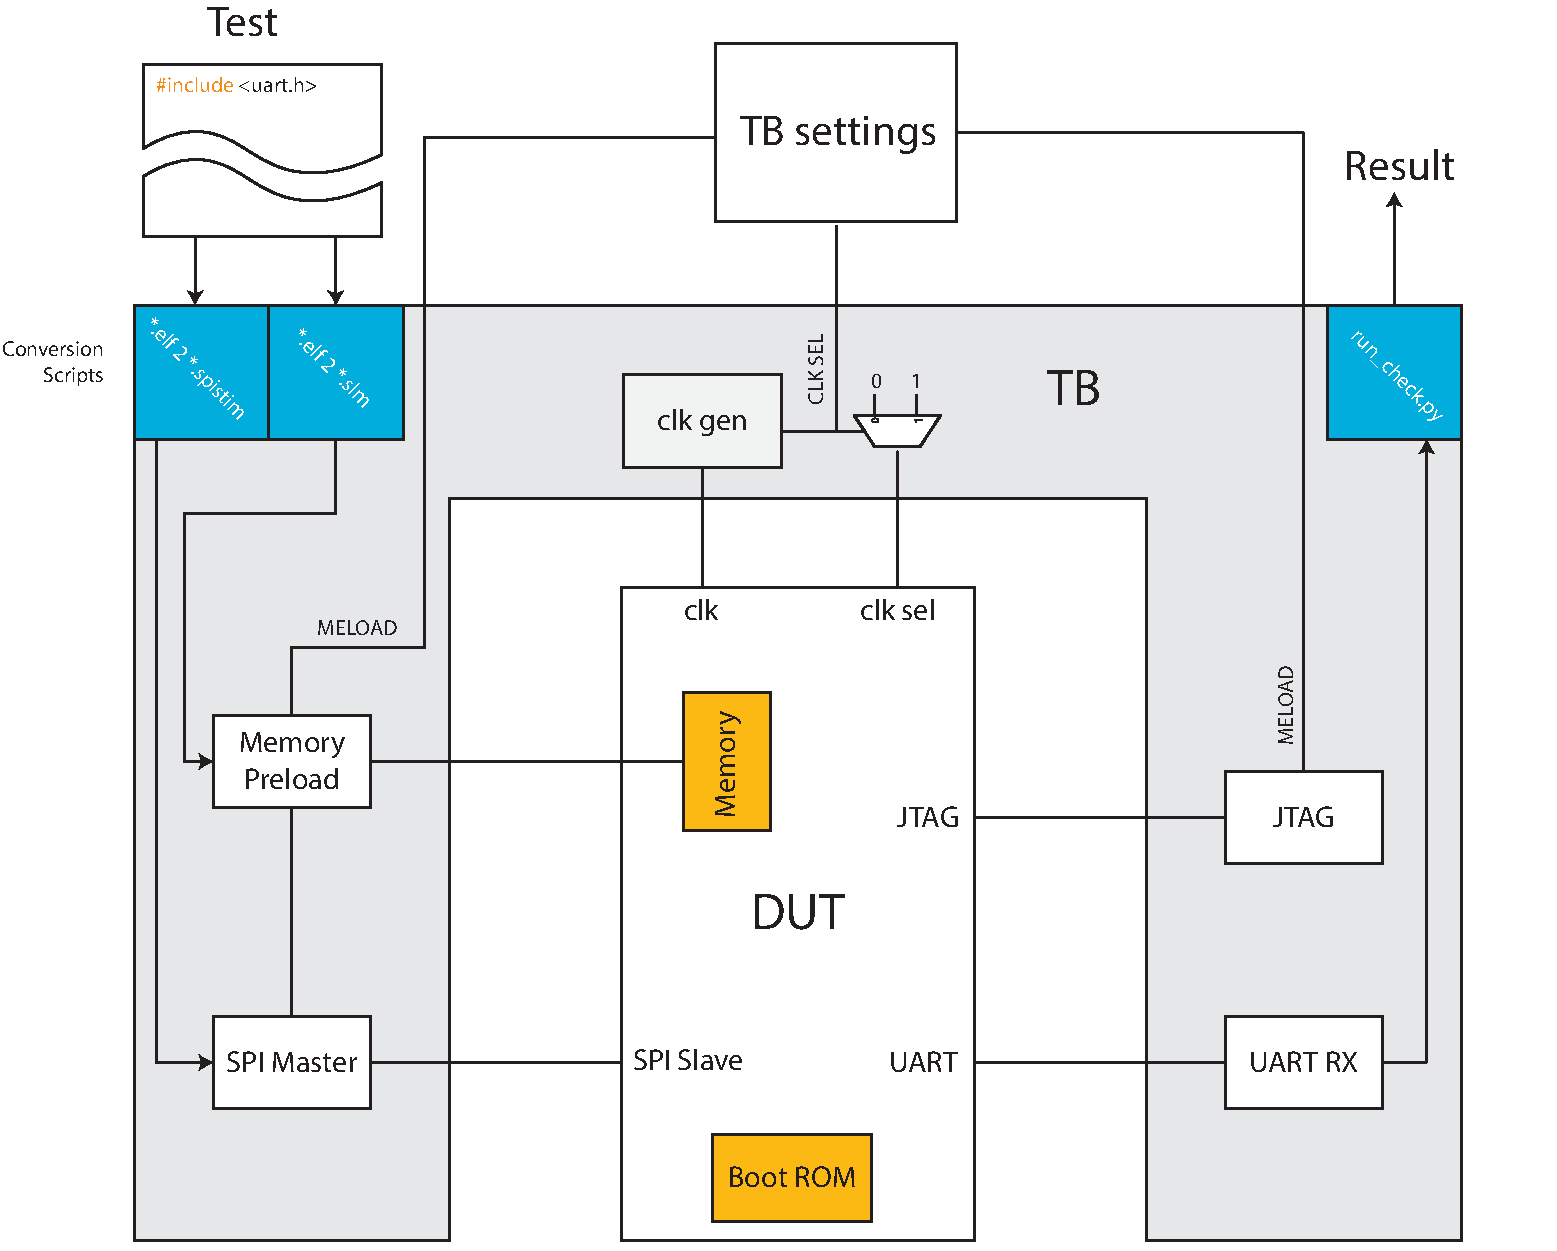
\includegraphics[width=\linewidth]{./figures/test_environment}
  \caption{Functional verification setup.}
  \label{fig:func_ver}
\end{figure}

\subsection{Design for Testability (DFT)}

The RAM's input is bypassed in test mode in order to enable scan testing the combinatorial logic around the RAM. This is especially important for the RAM2AXI interfaces which allow operations on the bare memory. Furthermore, in order to observe the address pins of the RAM observation registers for the RAM address port have been added. The area overhead is small since Synopsys uses some sophisticated techniques to, on the one hand reuse the observation registers for both the instruction and the data RAM and on the other hand, only a few registers are necessary to make the signals of interest observable. \\
The memories itself will be tested with direct access through the JTAG interface. \\
The FLL has a dedicated DFT structure featuring a ScanEnable, ScanIn and ScanOut port. Until now the FLL is not part of one of the scan chains. \\
The current DFT numbers are related to post synthesis netlists. In a first run, a couple of weeks ago, I was able to achieve a bit more than 99 \% test coverage. While in the latest runs, most probably related to the newly instantiated pad frame and the FLL, test coverage deteriorated a bit and I am at 97\% for the current design. \\


\begin{lstlisting}
     Uncollapsed Stuck Fault Summary Report
 -----------------------------------------------
 fault class                     code   #faults
 ------------------------------  ----  ---------
 Detected                         DT     351339
 Possibly detected                PT         68
 Undetectable                     UD       1267
 ATPG untestable                  AU       8065
 Not detected                     ND         99
 -----------------------------------------------
 total faults                            360838
 test coverage                            97.72%
 fault coverage                           97.38%
 -----------------------------------------------
\end{lstlisting}

\subsubsection{Automated Testpattern Generation}


\begin{figure}[tb]
  \centering
  \includegraphics[width=\linewidth]{./figures/pad_instaces_img_ord}
  \caption{Bonding diagram}
  \label{fig:bonding_diagram}
\end{figure}

\section{Timing}

%talk about timing and how timing closure was achieved. useful skew, skew general relate to RAM bank implementation

\section{Power}

% power analysis

Lowering power has always been a key driving factor for the PULP group. As a matter of fact power consumption has been a point of interest for \pulpino as well. Nevertheless due to \pulpino's simplicity we spare most of the power saving tricks used by PULP. 

In order to estimate power consumption I extended the current testbench to automatically trigger ModelSim's VCD dumps. Additionally I configured the CMake environment (for more information you may want to check the Getting Started Guide~\ref{sec:getting_started}) to have a distinct power target. This makes it particularly easy to run power estimations.

Although the whole design is getting compiled with clock gating enabled it turned out that the peripherals were dissipating a lot of power. Considering that I decided to implement more extensive manual clock gating. Concretely I employed a distinct clock gating control register into the APB \pulpino peripheral. This register allows for clock gating every peripheral separately without relying on Synopsis automatic clock gating insertion alone.

Another measure I took, in order to lower power, was the usage of standard cells with different voltage threshold. The standard cells in UMC 65 technology come in three different flavors in terms of threshold voltage (VT), depending on the needs of the designer. Cells that have a high threshold voltage have slower transition times (the time needed to switch from one voltage level of logic 0/1 to the voltage level of 1/0) but do dissipate less leakage current (power dissipated by the cell in absence of any switching activity) than standard cells with lower threshold voltages. The other two types of standard cells are regular VT and low VT cells. The latter are switching faster but dissipate way more leakage current.

Depending on the requirements of the standard cell needed for a certain part of the design, the synthesis tool can decide which standard cell it wants to use. It will of course always try to meet the speed requirement constrained by the designer but on the other hand it will also optimize in terms of leakage power dissipated.

\section{Results}

This section deals about the results I've received during design time.

\subsection{Power}

For the time being I conducted three different measurements that are mostly representative for Imperio's application context.

\begin{enumerate}
    \item Interrupt Test: The core is clock gated most of the time in this scenario. It is woken up periodically and performs an UART transaction when it wakes up.
    \item Hello World: Trivial UART output. The core is not put to a particular low power state. Most of the operations are memory operations (instruction and data fetches).
    \item Matrix Multiplication: Computational intensive operation. The core needs to fetch a lot of data from the memories and performing computational costly operations, like multiplications and additions on it. This case should be representative for high density computation. 
\end{enumerate}

Power consumption can be split up into the following three components~\cite{Kaeslin08}:
\begin{itemize}
    \item Internal power $P_{int}$: power dissipated for charging and discharging the cell's internal capacitances.
    \item Switching power $P_{ext}$: this amounts to the power that gets dissipated for charging external load capacitances (input capacitance of driven cell plus wire capacitances) that are connected to the cell's output(s).
    \item Leakage power $P_{leak}$: power dissipated by the cell in absence of switching activity.
\end{itemize}
The total power dissipated by the circuit is the sum of these:
\[
    P_{tot} = P_{int} + P_{ext} + P_{leak}
\]
All power simulations where performed at 500 MHz, 1.2 V and 25 \textdegree C. Detailed results are depicted in table~\ref{tab:power}.

\begin{table}[htbp]
 \caption{Power Results (UMC65 - LVT 1.2V) @ 2ns, 25 \textdegree C}
 \label{tab:power}
\begin{tabularx}{\textwidth}{|X||r|r||r|r||r|r||r|}
  \hline
  \textbf{Test} & $P_{int}$& \% & $P_{ext}$ &  \% & $P_{leak}$ &  \% & $P_{tot}$\\ \hline
Interrupt Test & 7.10 & 57.84 & 5.00 &  40.64 & 0.17 & 1.52 & 12.28 \\ \hline
Hello World & 19.80 & 59.64 & 13.25 & 39.88 & 0.19 & 0.56 & 33.23 \\ \hline
Mat. Mul. & 32.00 & 60.00 & 21.17 & 39.68 & 0.19 & 0.35 & 53.35 \\ \hline
  \end{tabularx}
  \end{table}


\section{Area}

On the final design there is approximately 25\% core area left (on a ninth module). Detailed area results are listed in figure~\ref{fig:area}. Note that the RAMs are no longer listed as a separate design entry as they are completely ungrouped for better synthesis results. Pad instances do not show up as seperate design entries since they are not over 1 kGE alone, but accumulated they are a significant part of the overall area.

% ------- Python generated ---------
\begin{figure}[ht!]
\centering
\begin{tabularx}{\textwidth}{Xrrrrrr}
\textbf{Entity} &  \multicolumn{3}{l}{\textbf{Total Cells (kGE)}}  &  \multicolumn{3}{l}{\textbf{\% Total}}  \\\hline
imperio&700&&&100.0&&\\
pulpino\_i&500&&&73.1&&\\
$\quad$axi\_interconnect\_i&&6&&&1.0&\\
$\quad\quad$axi\_node\_i&&&6&&&1.0\\
$\quad\quad$others &&&0&&&0\\
$\quad$clk\_rst\_gen\_i&&12&&&1.8&\\
$\quad\quad$others &&&0&&&0.0\\
$\quad$core\_region\_i&&400&&&63.6&\\
$\quad\quad$RISCV\_CORE&&&40&&&5.8\\
$\quad\quad$adv\_dbg\_if\_i&&&5&&&0.8\\
$\quad\quad$axi\_slice\_core2axi&&&2&&&0.4\\
$\quad\quad$data\_mem\_axi\_if&&&5&&&0.8\\
$\quad\quad$instr\_mem\_axi\_if&&&5&&&0.8\\
$\quad\quad$others &&&0&&&0.0\\
$\quad$peripherals\_i&&50&&&6.8&\\
$\quad\quad$apb\_event\_unit\_i&&&3&&&0.5\\
$\quad\quad$apb\_gpio\_i&&&3&&&0.5\\
$\quad\quad$apb\_i2c\_i&&&1&&&0.2\\
$\quad\quad$apb\_pulpino\_i&&&2&&&0.3\\
$\quad\quad$apb\_spi\_master\_i&&&8&&&1.2\\
$\quad\quad$apb\_timer\_i&&&3&&&0.5\\
$\quad\quad$axi2apb\_i&&&1&&&0.2\\
$\quad\quad$axi\_spi\_slave\_i&&&8&&&1.3\\
$\quad\quad$i\_apb\_uart&&&14&&&2.1\\
$\quad\quad$others &&&0&&&0.0\\
\end{tabularx}
\caption{Area estimates (UMC65 - LVT 1.2V) @ 1.3ns - 1 GE = 1.44 \textmu m$^2$}
\label{fig:area}
\end{figure}
% ------- Python generated ---------

% If you only have very few results, it might be a better approach to
% insert them into this chapter (instead of putting the results into a
% separate one).


